\section{Testing Methodologies}\label{sec:methodology}

We describe two experiments testing OpenCL configurations using our approach. The first is results from unstructured, opportunistic testing of OpenCL implementations while developing CLgen, resulting in XX bug reports to OpenCL vendors. The second is a direct comparison of our approach to CLSmith, the current state-of-the-art in OpenCL test case generation.

% \subsection{Parameters}
% \begin{table}[t!]
  \scriptsize %
  \centering %
  \rowcolors{2}{white}{gray!25}
  \begin{tabular}{rlll}
\toprule
 Dataset Size &   Global size &  Local size & Optimizations \\
\midrule
          256 &     (1, 1, 1) &   (1, 1, 1) &           off \\
          256 &     (1, 1, 1) &   (1, 1, 1) &            on \\
         4096 &  (128, 16, 1) &  (32, 1, 1) &           off \\
         4096 &  (128, 16, 1) &  (32, 1, 1) &            on \\
\bottomrule
\end{tabular}

  \caption{Test case parameters.}
  \label{tab:cldrive-params}
\end{table}

% Table~\ref{tab:cldrive-params}. 

%\subsection{Classifying test cases}
%
%\cc{Use the results of difftest to determine whether the input sample was formed, well-typed, free from UB, etc. Plot ratio of CLgen and CLSmith outputs according to classifications (CLSmith should be all perfect).}
%
%\begin{enumerate}
%  \item Ill-formed ASCII sequence. The test case contains syntax errors preventing compilation.
%  \item Well-formed program.
%  \item Well-typed program.
%  \item Standard-conformant OpenCL program. The program
%\end{enumerate}

\subsection{Test Case Execution}

\begin{figure}
  \centering %
  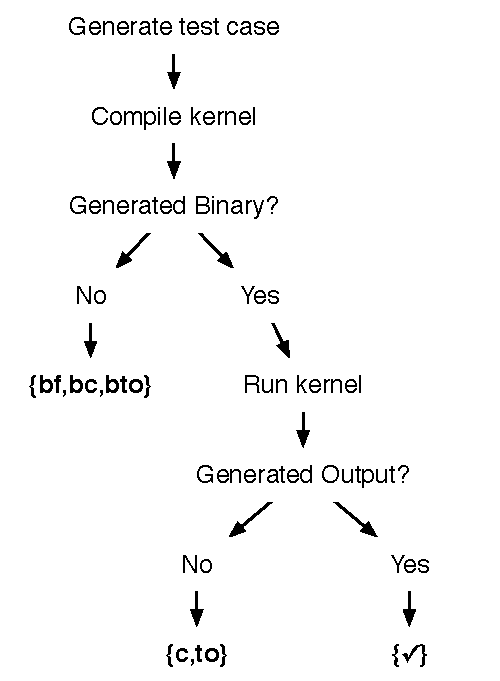
\includegraphics[width=\columnwidth]{img/test_process}%
  \caption{%
  	Test case execution, and possible outcomes. For each test case, a $(+,-)$ pair of outcomes is produced.%
  }%
  \label{fig:test-process} %
\end{figure}



Figure~\ref{fig:test-process} shows the methodology for determining the outcomes of a single test case.

In prior work we required that synthesized programs be well formed and compute \emph{useful work}. For the purpose of testing compilers, we discarded these requirements. Instead, we demand that the behavior of test cases is \emph{portable} and \emph{reproducible}. In some respects this simplifies the execution process. The possible outcomes for a test case are a build failure (\textbf{bf}), build crash (\textbf{bc}), runtime crash (\textbf{c}), or pass (\textbf{\cmark}). A \textbf{bf} occurs when compilation of a kernel fails, usually accompanied by an error message. A \textbf{bc} outcome occurs when the compiler crashes. In~\cite{Lidbury2015a}, the authors do not distinguish between compiler crashes and build failures. A \textbf{c} outcome occurs when the program crashes during execution. The \textbf{bto} and \textbf{to} outcomes occur when the program compilation or execution time out, respectively. As in previous work, we do not guarantee that generated programs time out, finding that XX\% of programs do not.

There are six possible outcomes of a test case execution:
%
\begin{enumerate}
	\item \textbf{bf} \emph{Build failure} Online compilation of OpenCL program fails, whereas the majority of configurations produce a binary.
	\item \textbf{bc} \emph{Build crash} Compilation of program fails due to compiler crahs.
	\item \textbf{bto} \emph{Build timeout} Online compilation of OpenCL exceeds a timeout of 60 seconds.
	\item \textbf{c} \emph{Runtime crash} One or more OpenCL API calls return an error status during the program execution, or the program crashes.
	\item \textbf{to} \emph{Runtime timeout} Program execution exceeds the timeout of 60 second.
	\item \textbf{\cmark} \emph{Completion} The program terminates gracefully and produces an output.
\end{enumerate}


\subsection{Voting Heuristics for Differential Testing}

In~\cite{Lidbury2015a}, a configuration is determined to have produced a wrong code result for a kernel if there is a majority of at least 3 among the non-\{\textbf{bf},\textbf{c},\textbf{to}\} results for the kernel, and the configuration yields a non-\{\textbf{bf},\textbf{c},\textbf{to}\} result that disagrees with the majority.

A majority exists if there are at least 6 non-bc results for the kernel, and of these $n$ non-bc configurations, at least $\ceil{n/2}$ configurations have the same outcome. Majority outcome $\mu$. For \cmark outcomes, the output of the program is used.

%
\begin{enumerate}
	\item \textbf{w} \emph{Wrong code} Program terminates gracefully, but computes a result which differs from the majority output.
	\item \textbf{bf} \emph{Build failure} Online compilation of OpenCL program fails, whereas the majority of configurations produce a binary.
	\item \textbf{bto} \emph{Build timeout} Online compilation of OpenCL exceeds a timeout of 60 seconds, whereas the majority of configurations produce a binary.
	\item \textbf{c} \emph{Runtime crash} One or more OpenCL API calls return an error status during the program execution, or the program crashes.
	\item \textbf{to} \emph{Runtime timeout} Program execution exceeds the timeout of 60 second, whereas the majority of configurations produce an output.
\end{enumerate}


\begin{table}
	\scriptsize %
	\centering %
	\begin{tabular}{ c|ccc }
		\toprule
		 & \multicolumn{3}{c}{\textbf{Minority outcome}} \\
		 & \textbf{bf} & \textbf{c} & \textbf{\cmark} \\
		\midrule
		\textbf{bf} & \cmark & ? & ? \\
		\textbf{c} & c & \cmark & ? \\
		\textbf{\cmark} & bf & c & \cmark \\
		\bottomrule
	\end{tabular}
	\caption{Voting heuristics to determine the classification of results based on the majority outcome (rows) \cc{wtf is this\ldots}}
	\label{tab:voting-heuristics}
\end{table}

\paragraph{Floating points} The OpenCL 1.2 specification permits acceptable error bounds (ULP) for floating point operations and builtin functions. Some operations like addition, subtraction, and multiplication are precise; divide permits a small error, and builtins vary widely. Thus two implementation may give different answers that both fit within the allowed ranges (and because errors propagate through operations it's hard to even describe the ULP on the final output). \texttt{half\_} functions permit large error bounds. \texttt{native\_} functions have ``implementation defined'' error bounds. TODO: Denormal numbers may optionally be pushed to zero.

\cc{If we difftest across floats:}
CSmith, and by extension, CLSmith, do not support floating point operations. In our observations with testing using CLSmith (described in Section~\ref{sec:vs_clsmith}), we observed that in cases of wrong-code bugs, the computed values are usually entirely incorrect, not only marginally different. We hypothesized that by allowing relaxed comparisons between floating point values, we could still differential test. We permit a margin of deviation for floating point comparisons. This means that if a compiler were to emit wrong code which changes the computed value only subtly, we may miss it; though we have no reason to suggest that such a case is any more likely than a wrong code bug leading the compiler to produce exactly the same output, which neither we or any prior work have noted.

\cc{If we ignore floats:}
Given that not all vendors provide bounds for floating point imprecision, we excluded kernels containing floating points from the wrong-code check. Given knowledge about hardware imprecision, it would be possible to compute threshold for floating point difftests.
% Section 7.4 of OpenCL 1.2 spec.